\section{Development and Implementation}
\subsection{Introduction to Languages}
\subsubsection{Java}
\begin{figure}[ht]
\centering

\includegraphics[scale=0.5]{input/images/java.png}
\caption{Java Logo}
\end{figure}
Java programming language was originally developed by Sun Microsystems which was initiated by James
Gosling and released in 1995 as core component of Sun Microsystems' Java platform. The latest release of
the Java Standard Edition is Java SE 8. With the advancement of Java and its widespread popularity,
multiple configurations were built to suit various types of platforms. For example: J2EE for Enterprise
Applications, J2ME for Mobile Applications.


\subsection{Python}

\begin{figure}[ht]
\centering

\includegraphics[scale=0.5]{input/images/py.png}
\caption{Python Logo}
\end{figure}
Python is a high-level, interpreted, interactive and object-oriented scripting language. Python is designed
to be highly readable. It uses English keywords frequently where as other languages use punctuation, and
it has fewer syntactical constructions than other languages.
\subsection{Javascript}
\begin{figure}[!ht]
\centering

\includegraphics[width=0.3\textwidth]{input/images/JS.png}
\caption{Javascript logo}
\hspace{-1.5em}
\end{figure}

JavaScript (/ˈdʒɑːvəˌskrɪpt/) is a high-level, dynamic, untyped, and interpreted programming language. It has been standardized in the ECMAScript language specification. Alongside HTML and CSS, it is one of the three essential technologies of World Wide Web content production; the majority of websites employ it and it is supported by all modern web browsers without plug-ins. JavaScript is prototype-based with first-class functions, making it a multi-paradigm language, supporting object-oriented, imperative, and functional programming styles. It has an API for working with text, arrays, dates and regular expressions, but does not include any I/O, such as networking, storage or graphics facilities, relying for these upon the host environment in which it is embedded.

\subsection{SQLite}
\begin{figure}[ht]
\centering

\includegraphics[scale=0.5]{input/images/sq.png}
\caption{SQLite Logo}
\end{figure}
SQLite is an in-process library that implements a self-contained, serverless, zero-configuration,
transactional SQL database engine. It is a database, which is zero-configured, which means like other
databases you do not need to configure it in your system. SQLite engine is not a standalone process like
other databases, you can link it statically or dynamically as per your requirement with your application.
SQLite accesses its storage files directly.
\section{Any other Supporting Languages or tools}
\subsection{Android}
\begin{figure}[ht]
\centering

\includegraphics[scale=0.5]{input/images/android.png}
\caption{Android Logo}
\end{figure}
Android is a mobile operating system developed by Google, based on the Linux kernel and designed
primarily for touchscreen mobile devices such as smartphones and tablets. Android's user interface is
mainly based on direct manipulation, using touch gestures that loosely correspond to real-world actions,
such as swiping, tapping and pinching, to manipulate on-screen objects, along with a virtual keyboard for
text input. 
\subsection{Android Studio}
\begin{figure}[ht]
\centering

\includegraphics[scale=0.5]{input/images/as.png}
\caption{Android Studio Logo}
\end{figure}
Android Studio is the official integrated development environment (IDE) for Android platform
development. Android Studio provides the fastest tools for building apps on every type of Android device.
\subsection{Strophe.js}
Strophe.js is an XMPP library for JavaScript. Its primary purpose is to enable web-based, real-time XMPP
applications that run in any browser. This library uses either Bidirectional-streams Over Synchronous
HTTP (BOSH) to emulate a persistent, stateful, two-way connection to an XMPP server or alternatively
Web Sockets.
\subsection{BOSH (protocol)}
Bidirectional-streams Over Synchronous HTTP (BOSH) is a transport protocol that emulates a bidirectional
stream between two entities (such as a client and a server) by using multiple synchronous HTTP
request/response pairs without requiring the use of polling or asynchronous chunking.
\subsection{Ejabberd}
\begin{figure}[ht]
\centering

\includegraphics[scale=0.5]{input/images/ej.png}
\caption{Ejabberd Logo}
\end{figure}
ejabberd is an XMPP application server, written mainly in the Erlang programming language. It can run
under several Unix-like operating systems such as Mac OS X, GNU/Linux, FreeBSD, NetBSD, OpenBSD
and OpenSolaris. Additionally, ejabberd can run under Microsoft Windows. The name ejabberd stands for
Erlang Jabber Daemon (Jabber being a former name for XMPP) and is written in lowercase only, as is
common for daemon software.
\subsection{Errbot}
\begin{figure}[ht]
\centering

\includegraphics[scale=0.5]{input/images/er.png}
\caption{Errbot Logo}
\end{figure}
Errbot is a chatbot, a daemon that connects to your favourite chat service and brings your tools into the
conversation. The goal of the project is to make it easy for you to write your own plugins, so you can make
it do whatever you want: a deployment, retrieving some information online, trigger a tool via an API, troll
a co-worker. Errbot is being used in a lot of different contexts: chatops (tools for devops), online gaming
chatrooms like EVE, video streaming chatrooms like livecoding.tv, home security, etc.
\subsection{SleekXMPP}
SleekXMPP is an elegant Python library for XMPP (aka Jabber, Google Talk, etc). SleekXMPP is an MIT licensed XMPP library for Python 2.6/3.1+, and is featured in examples in XMPP: The Definitive Guide
by Kevin Smith, Remko Tronçon, and Peter Saint-Andre. If you’ve arrived here from reading the Definitive
Guide, please see the notes on updating the examples to the latest version of SleekXMPP.


\section{Ubuntu: An open source OS}
\begin{figure}[!ht]
\centering

\includegraphics[width=0.3\textwidth]{input/images/ubu.png}
\caption{Ubuntu}
\hspace{-1.5em}
\end{figure}

During my training, I also got familiar with a great and open source Operating System, Ubuntu. Firstly, it was quite difficult for a regular MS Windows user to port to Ubuntu. I did all of my project work using this vast operating system. 
Ubuntu is a Debian-based Linux operating system, with Unity as its default desktop environment. It is based on free software and named after the Southern African philosophy of ubuntu (literally, "human-ness"), which often is translated as "humanity towards others" or "the belief in a universal bond of sharing that connects all humanity".\\

Ubuntu's goal is to be secure "out-of-the box". By default user's programs run with low privileges and cannot corrupt the operating system or other user's files. For increased security, the sudo tool is used to assign temporary privileges for performing administrative tasks, which allows the root account to remain locked and helps prevent inexperienced users from inadvertently making catastrophic system changes or opening security holes.\\




\begin{figure}[ht]
\centering 
\includegraphics[scale=1]{input/images/doxygen.jpeg}
\caption{Doxygen logo}
\end{figure}
\noindent Doxygen is a documentation generator, a tool for writing software reference 
documentation. The documentation is written within code, and is thus 
relatively easy to keep up to date. Doxygen can cross reference 
documentation and code, so that the reader of a document can easily 
refer to the actual code.

Doxygen supports multiple programming languages, especially C++, C, 
C\#, Objective-C, Java, Python, IDL, VHDL, Fortran and PHP.[2] Doxygen
 is free software, released under the terms of the GNU General Public 
License.\\

\section{Introduction To Doxygen}
\begin{itemize}
\item Requires very little overhead from the writer of the documentation. 
Plain text will do, Markdown is support, and for more fancy or structured 
output HTML tags and/or some of doxygen's special commands can be used.
\item Cross platform: Works on Windows and many Unix flavors (including 
Linux and Mac OS X).
\item Comes with a GUI frontend (Doxywizard) to ease editing the options 
and run doxygen. The GUI is available on Windows, Linux, and Mac OS X.
\item Automatically generates class and collaboration diagrams in HTML 
(as clickable image maps) and $\mbox{\LaTeX}$ (as Encapsulated PostScript 
images).
\item Allows grouping of entities in modules and creating a hierarchy 
of modules.
\item Doxygen can generate a layout which you can use and edit to change 
the layout of each page.
\item Can cope with large projects easily.
\end{itemize}
\subsection{Installation of Doxygen}
Doxygen can be installed using following commands:\\

\hspace{4pt} \$ git clone https://github.com/doxygen/doxygen.git

\hspace{4pt} \$ cd doxygen

\hspace{4pt} \$ ./configure

\hspace{4pt} \$ make






\section{Introduction to \LaTeX}

\LaTeX, I had never heard about this term before doing this project,
but when I came to know about it's features, found it excellent. 
\LaTeX{ is a document markup language and document preparation system for the \TeX{} 
typesetting program. Within the typesetting system, its name is styled 
as \LaTeX.

\begin{figure}[!ht]
\centering
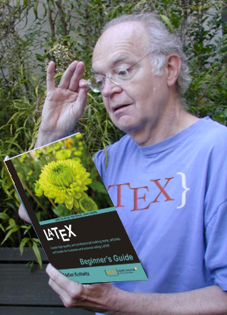
\includegraphics[width=0.3\textwidth]{input/images/donald.png}                   
\caption{Donald Knuth, Inventor Of \TeX{} 
typesetting system}
\hspace{-1.5em}
\end{figure}

Within the typesetting system, its name is styled as \LaTeX. The term 
\LaTeX{} refers only to the language in which documents are written, 
not to the editor used to write those documents. In order to create a 
document in \LaTeX, a .tex file must be created using some form of text 
editor. While most text editors can be used to create a \LaTeX{} document, 
a number of editors have been created specifically for working with \LaTeX.

\LaTeX{} is most widely used by mathematicians, scientists, 
engineers, philosophers, linguists, economists and other scholars in 
academia. As a primary or intermediate format, e.g., translating DocBook 
and other XML-based formats to PDF, \LaTeX{} is used because of the 
high quality of typesetting achievable by \TeX. The typesetting system 
offers programmable desktop publishing features and extensive facilities 
for automating most aspects of typesetting and desktop publishing, 
including numbering and cross-referencing, tables and figures, 
page layout and bibliographies.

\LaTeX{} is intended to provide a high-level language that
accesses the power of \TeX. \LaTeX{} essentially comprises a
collection of \TeX{} macros and a program to process \LaTeX documents. 
Because the \TeX{} formatting commands are very low-level, it is usually 
much simpler for end-users to use \LaTeX{}.


\subsection{Typesetting}
In preparing a \LaTeX{} document, the author 
specifies the logical structure using familiar concepts such as 
chapter, section, table, figure, etc., and lets the \LaTeX{} system 
worry about the presentation of these structures. It therefore 
encourages the separation of layout from content while still allowing 
manual typesetting adjustments where needed. 

\begin{verbatim}
\documentclass[12pt]{article}
\usepackage{amsmath}
\title{\LaTeX}
\date{}
\begin{document}
  \maketitle 
  \LaTeX{} is a document preparation system 
  for the \TeX{} typesetting program.
\end{document}
\end{verbatim}

\begin{figure}[!ht]
\centering
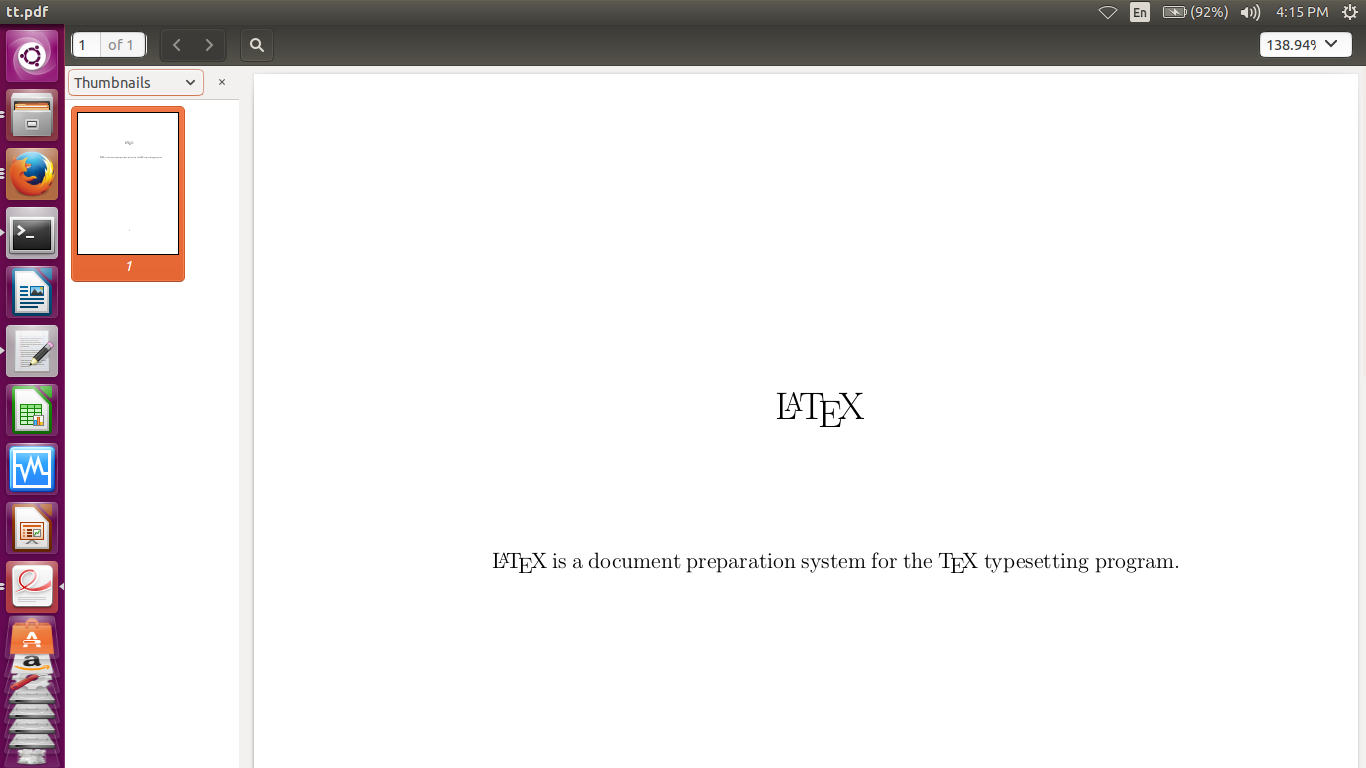
\includegraphics[width=0.7\textwidth]{input/images/la.png}
\caption{Output of the avove program}
\hspace{-1.5em}
\end{figure}


\section{Introduction to Github}
\begin{figure}[!ht]
\centering

\includegraphics[width=0.3\textwidth]{input/images/github.jpg}                   
\caption{Github Logo}
\hspace{-1.5em}
\end{figure}
\leavevmode\\
GitHub is a Git repository web-based hosting service which offers all of the functionality of Git as well as adding many of its own features. Unlike Git which is strictly a command-line tool, Github provides a web-based graphical interface and desktop as well as mobile integration. It also provides access control and several collaboration features such as wikis, task management, and bug tracking and feature requests for every project.\\

GitHub offers both paid plans for private repo handle everything from small to very large projects with speed and efficiency. ositories, and free accounts, which are usually used to host open source software projects. As of 2014, Github reports having over 3.4 million users, making it the largest code host in the world.\\

GitHub has become such a staple amongst the open-source development community that many developers have begun considering it a replacement for a conventional resume and some employers require applications to provide a link to and have an active contributing GitHub account in order to qualify for a job.\\

The Git feature that really makes it stand apart from nearly every
other Source Code Management (SCM) out there is its branching model.\\
\\
Git allows and encourages you to have multiple local branches that can
be entirely independent of each other. The creation, merging, and
deletion of those lines of development takes seconds.\\ \\
This means that you can do things like:
\begin{itemize}
\item Frictionless Context Switching.\\ Create a branch to try out an
idea, commit a few times, switch back to where you branched from,
apply a patch, switch back to where you are experimenting, and merge
it in.
\item Role-Based Code lines. \\ Have a branch that always contains only
what goes to production, another that you merge work into for testing,
and several smaller ones for day to day work.
\item Feature Based Work flow. \\ Create new branches for each new
feature you're working on so you can seamlessly switch back and forth
between them, then delete each branch when that feature gets merged
into your main line.
\item Disposable Experimentation.\\  Create a branch to experiment in,
realize it's not going to work, and just delete it - abandoning the
work—with nobody else ever seeing it (even if you've pushed other
branches in the meantime).
\end{itemize}
Notably, when you push to a remote repository, you do not have to push
all of your branches. You can choose to share just one of your
branches, a few of them, or all of them. This tends to free people to
try new ideas without worrying about having to plan how and when they
are going to merge it in or share it with others.\\ \\
There are ways to accomplish some of this with other systems, but the
work involved is much more difficult and error-prone. Git makes this
process incredibly easy and it changes the way most developers work
when they learn it.

\subsection{What is Git?}
\begin{figure}[!ht]
\centering

\includegraphics[width=0.3\textwidth]{input/images/git.jpg}                   
\caption{Git Logo}
\hspace{-1.5em}
\end{figure}
Git is a distributed revision control and source code management (SCM) system with an emphasis on speed, data integrity, and support for distributed, non-linear workflows. Git was initially designed and developed by Linus Torvalds for Linux kernel development in 2005, and has since become the most widely adopted version control system for software development.\\

As with most other distributed revision control systems, and unlike most client–server systems, every Git working directory is a full-fledged repository with complete history and full version-tracking capabilities, independent of network access or a central server. Like the Linux kernel, Git is free and open source software distributed under the terms of the GNU General Public License version 2 to handle everything from small to very large projects with speed and efficiency.\\

Git is easy to learn and has a tiny footprint with lightning fast performance. It outclasses SCM tools like Subversion, CVS, Perforce, and ClearCase with features like cheap local branching, convenient staging areas, and multiple workflows.\\

\subsection{Installation of Git}

Installation of git is a very easy process.
The current git version is: 2.0.4.
Type the commands in the terminal:\\\\
\emph{
\$ sudo apt-get update\\\\
\$ sudo apt-get install git\\\\}
This will install the git on your pc or laptop.

\subsection{Various Git Commands}

Git is the open source distributed version control system that facilitates GitHub activities on your laptop or desktop. The commonly used Git command line instructions are:-\\

\subsubsection{Create Repositories}
Start a new repository or obtain from an exiting URL

\begin{description}

\item [\$ git init [ project-name]]\\
Creates a new local repository with the specified name
\item [\$ git clone [url]]\\
Downloads a project and its entire version history\\

\end{description}


\subsubsection{Make Changes}
Review edits and craft a commit transaction

\begin{description}

\item [\$ git status] \leavevmode \\
Lists all new or modified files to be committed

\item [\$ git diff] \leavevmode \\
Shows file differences not yet staged

\item [\$ git add [file]]\\
Snapshots the file in preparation for versioning

\item [\$ git commit -m "[descriptive message]"]\\
Records file snapshots permanently in version history\\

\end{description}


\subsubsection{Group Changes}
Name a series of commits and combine completed efforts

\begin{description}

\item [\$ git branch] \leavevmode \\
Lists all local branches in the current repository

\item [\$ git branch [branch-name]]\\
Creates a new branch

\item [\$ git checkout [branch-name]]\\
Switches to the specified branch and updates the working directory

\item [\$ git branch -d [branch-name]]\\
Deletes the specified branch\\

\end{description}


\subsubsection{Synchronize Changes}
Register a repository bookmark and exchange version history

\begin{description}

\item [\$ git fetch [bookmark]]\\
Downloads all history from the repository bookmark

\item [\$ git merge [bookmark]/[branch]]\\
Combines bookmark’s branch into current local branch

\item [\$ git push [alias][branch]]\\
Uploads all local branch commits to GitHub

\item [\$ git pull] \leavevmode \\
Downloads bookmark history and incorporates changes

\end{description}



%\section{Introduction to Reveal-js \& Reveal-md}
\begin{figure}[!ht]
\centering

\includegraphics[width=0.3\textwidth]{input/images/reveal.png}                   
\caption{MD \& JS}
\hspace{-1.5em}
\end{figure}
Reveal-js is one of the framework of Javascript. This can be used for presentations purpose.\\
Now before going to reveal-md lets talk about some fundamental things.\\
What is a Markup language?\\
Markup languages are designed for the processing, definition and presentation of text. The language specifies code for formatting, both the layout and style, within a text file. HTML and Markdown  is an example of a widely known and used markup language.\\
Markdown is a lightweight Markup Language with simple plain text formatting syntax designed so that it can be converted to HTML and many other formats. It is created by  John Gruber. It had '.md' or '.markdown' extention.\\
"Markdown is a text-to-HTML conversion software tool written in Perl for web writers."\\
Moreover, to enable markdown feature of reveal.js, we need reveal-md. The Markdown feature of reveal.js is awesome, and has an easy (and configurable) syntax to separate slides. Use three dashes surrounded by two blank lines.\\
\subsection{Installation of reveal-md}
Installation of reveal-md is a very easy process.
Type the commands in the terminal:\\\\
\emph{
\$ sudo apt-get install npm\\\\
\$ sudo apt-get install nodejs-legacy\\\\
\$ sudo npm install -g reveal-md\\\\}
This will install reveal-md on your pc or laptop.



\section{Working with Server}
\begin{figure}[!ht]
\centering

\includegraphics[width=0.3\textwidth]{input/images/ser.png}                   
\caption{Server Communication}
\hspace{-1.5em}
\end{figure}
I had done the whole project on ubuntu server and had also learnt about making your system a server.\\
What is a Remote Server?\\
In simple words its nothing much but a Computer that is not attached to a user’s keyboard but over which he or she has some degree of control (like can see data of that computer, can retrieve or send data etc.)\\
For going deep you need to know about ssh (Secure Shell).\\
I had done it using Mosh. There are few terms related to this :\\
\begin{itemize}
\item SSH: It is a Secure Socket Shell, is a network protocol that provides administrators with a secure way to access a remote computer.
\item MOSH: It is a software tool used to connect from a client computer to a server over the Internet, to run a remote terminal. 
\item Tmux: tmux is basically a terminal multiplexer. It is used so that within
one terminal window we can open multiple windows and split-views.
\item OpenSSH: It is a freely available version of the Secure Shell (SSH) protocol family of tools for remotely controlling or transferring files between computers. Traditional tools used to accomplish this is telnet which is not much secure.
\end{itemize}

In Unix, you can use SCP (the scp command) to securely copy files and directories between remote hosts without starting an FTP session or logging into the remote systems explicitly. \\
The scp command uses SSH to transfer data, so it requires a password.\\\\
Some of the useful commands in this for checking errors or for other purposes are: \\
\begin{itemize}
\item ll: This command is used to list the detail information of files and folder of a current directory. 
\item tail -f error.log: This is used for checking errors.
\item sudo apt-get install openssh-server
\item sudo vim /etc/ssh/sshdconfig \\
(To edit this as per your preferences. But first take a backup of this file for later default configurations if needed.)
\item sudo restart ssh \\
(To check your ssh daemon is running or not.)
\item ps -A | grep sshd \\
(This command should produce a line like this:

 some-number ? 00:00:00 sshd)
\item ssh user@hostip \\
(To enter into a remote server from some other system. )
\end{itemize}

 

%
\section{Python Django Framework}
\begin{figure}[!h]
\centering

\includegraphics[width=0.3\textwidth]{input/images/django.png}
\caption{Python Django Framework}
\hspace{-1.5em}
\end{figure}
Django is a web development framework that assists in building and maintaining quality web applications. Django helps eliminate repetitive tasks making the development process an easy and time saving experience. It is a Python web framework.\\\\
During the training period it's being used in making LuvLdh-Webapp. An app used for publish post on a facebook page using a Graph Facebook API with Python SDK-Development Kit.\\\\
Librehatti, an Enterprise Resource Planning(ERP) software is wholly build in Django with the vast extensive knowledge, datastructures. It is comletely open source available in Github. During training, it is being used to make a module Dispatch\_register and made GST enabled module.

%\section{OSM and its Components }
It is a collaborative project to create a free editable map of the world.
Now ,before beginning to make your own tile server, review some termonologies.
\begin{figure}[ht]
\centering 
\includegraphics[scale=0.6]{input/images/index.jpeg}
\caption{OpenStreetMap logo}
\end{figure}

\subsection{Benifits Of Own Tile Server}
 OSM map is accessible even when internet provider is down or when the power is off or both. It won't take much for to see the benefit of having your own piece of OpenStreetMap infrastructure.\\
Now it's turn to install, setup and configure all the necessary software to operate own tile server. All the instructions are illustrated in blog "https://amisha2016.wordpress.com"\\
These instructions build what OpenStreetMap calls a "tile server". That is, a computer that uses the OSM data set to create map images that are suitable for a website. Not every OpenStreetMap function is supported, but you will be able to create a local map, keep it up to date and customize it for your own purposes.
\begin{figure}[!ht]
\centering

\includegraphics[width=0.4\textwidth]{input/images/index.png}                   
\caption{Postgresql}
\hspace{-1.5em}
\end{figure}


\subsection{Postgresql / postgis}
PostGIS is a spatial database extender for PostgreSQL object-relational database. It adds support for geographic objects allowing location queries to be run in SQL.\\
Most spatial databases allow representing simple geometric objects such as points, lines and polygons. Some spatial databases handle more complex structures such as 3D objects, topological coverages, linear networks, and TINs.\\
On Ubuntu there are pre-packaged versions of both postgis and postgresql, so these can simply be installed via the Ubuntu package manager.\\
\subsection{Osm2pgsql}
 osm2pgsql is under active development and is best compiled from source.\\
osm2pgsql is a command-line based program that converts OpenStreetMap data to postGIS-enabled PostgreSQL databases.\\
Mapnik is an open source mapping toolkit for desktop- and server-based map rendering, written in C++.\\
One of its many users is the OpenStreetMap project (OSM), which uses it in combination with an Apache Web Server module (mod\_tile) to render tiles that make up the OSM ‘Slippy Map’ Layer.\\
\begin{figure}[!ht]
\centering
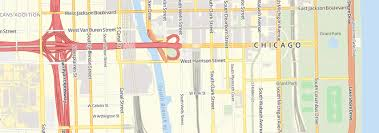
\includegraphics[width=0.7\textwidth]{input/images/bright.jpeg}                   
\caption{Openstreetmap-carto Style}
\hspace{-1.5em}
\end{figure}



\subsection{Openstreetmap-carto}
Openstreetmap-carto is a sensible starting point for quickly making beautiful maps based on an OpenStreetMap database. It is written in the Carto styling language and can be opened as a project in TileMill.\\
The style is still a work in progress and you are encouraged to use the issue tracker to note missing features or problems with the current implementation.\\
\subsection{OpenLayer.js}
OpenLayers makes it easy to put a dynamic map in any web page. It can display map tiles, vector data and markers loaded from any source. OpenLayers has been developed to further the use of geographic information of all kinds. It is completely free.\\
\subsection{Geographic Information Systems (GIS)}
GIS is a computer system for capturing, storing, checking, and displaying data related to positions on Earth’s surface. GIS can show many different kinds of data on one map. This enables people to more easily see, analyze, and understand patterns and relationships\\
The Global Positioning System (GPS) is a space-based navigation system that provides location and time information in all weather conditions, anywhere on or near the Earth where there is an unobstructed line of sight to four or more GPS satellites.\\


\section{Implementation of project}
\subsection{Architecture of project}
The following is the architecture of the Paigaam app. It contains the following modules:
\begin{figure}[ht]
\centering
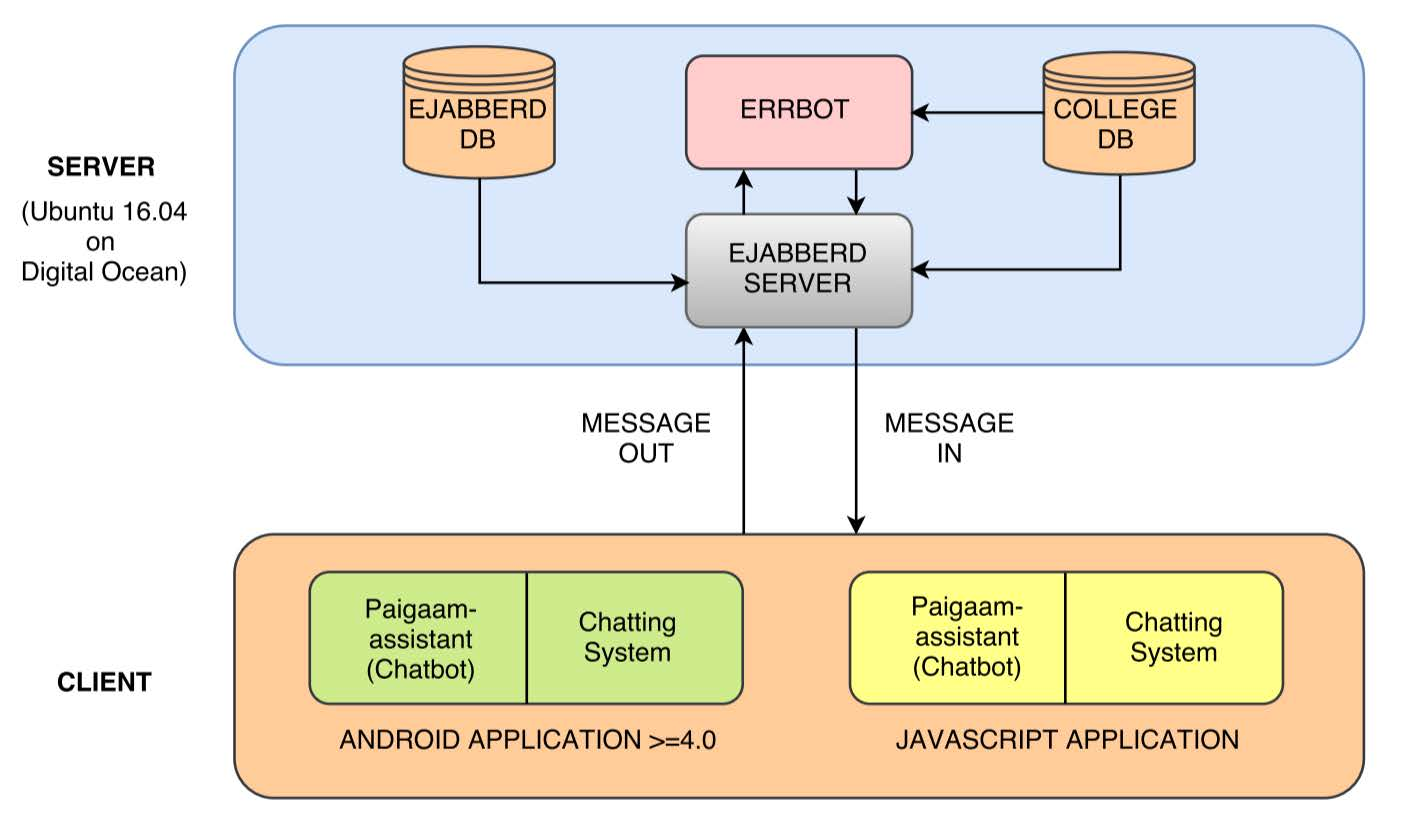
\includegraphics[scale=0.3]{input/images/im.png}
\caption{Paigaam Architecture}
\end{figure}\\
\noindent \textbf{Server}
The server is including the following modules:
\begin{itemize}
\item Ejabberd Server: Ejabberd is an XMPP server. It manages the user chats and user accounts and is
connected to ejabberd database.
\item Errbot: This is the brain behind the Paigaam assistant and is used to manage bot requests. It is
connected to a SQLite database.
\end{itemize}
\noindent \textbf{Client}
The client includes the following modules:
\begin{itemize}
\item Android App(Paigaam): The app has chatting features and a chatbot to answer user queries.
\item JavaScript Web App: This is the web based client of Paigaam.
\end{itemize}
\subsection{Working of the Paigaam-Assistant(Chatbot)}
The chatbot working is demonstrated in the following figure:
\begin{figure}[ht]
\centering
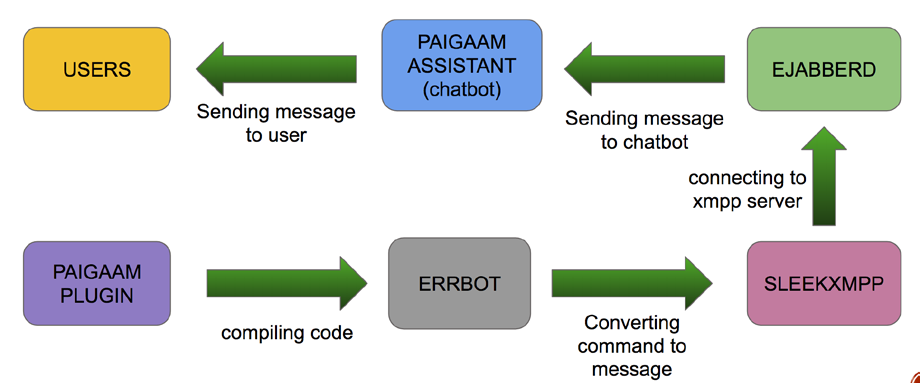
\includegraphics[scale=0.3]{input/images/aeb.png}
\caption{Paigaam-Assistant Working}
\end{figure}\\
\begin{itemize}
\item Errbot
The Errbot runs the python scripts and convert messages in XMPP format with the help of SleekXMPP.
\item SleekXMPP
SleekXMPP acts as an interface between Errbot and ejabberd and helps Errbot to send/receive messages
to/from the ejabberd XMPP server.
\item Ejabberd
The Ejabberd XMPP server is responsible for the messaging service of the app.
\item Paigaam Assistant
The Paigaam assistant(chatbot) sends and gets messages from the ejabberd server and shows them to the
users.
\item Users
The users interact with the chatbot to ask queries and get the answers.
\end{itemize}
\section{Test Cases}
The test cases include the testing of the Paigaam app, the Paigaam assistant(Chatbot) and as well as the
web client of Paigaam.
\subsection{Paigaam App}
\begin{enumerate}
\item Login\\
\noindent \textbf{Description:}
A non-registered user should not be able to successfully login into the app.\\
\noindent \textbf{Precondition:}
The user must not be registered with an email address and password.\\
\noindent \textbf{Test Steps:}
\begin{itemize}
\item Open the app.
\item Click on Options and then Manage Accounts.
\item Click on Add account icon.
\item Enter the wrong registered roll id and password and click on next.
\end{itemize}
\noindent \textbf{Expected Result:}
A message is displayed saying unauthorized password and/or server not found.\\
\begin{figure}[ht]
\centering
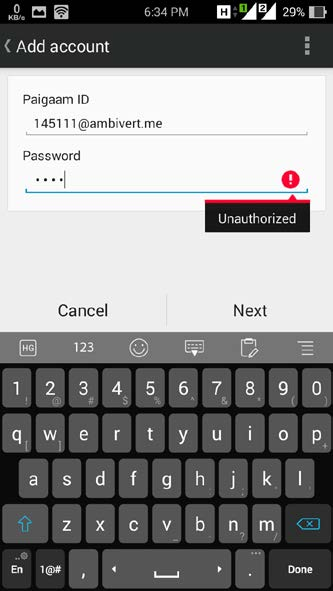
\includegraphics[scale=0.3]{input/images/s1.png}
\caption{Login Test ID and Password}
\end{figure}
\item Internet Connectivity\\
\noindent \textbf{Description:}
The user should be shown a message if the internet is not active.\\
\noindent \textbf{Precondition:}
Internet is not connected.\\
\noindent \textbf{Test Steps:}
\begin{itemize}
\item Open the app.
\item Click on Options and then Manage Accounts.
\end{itemize}
\noindent \textbf{Expected Result:}
A message is displayed saying No Connectivity under the account name.
\begin{figure}[ht]
\centering
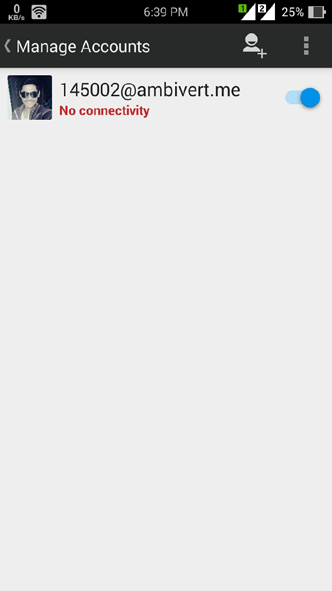
\includegraphics[scale=0.3]{input/images/s2.png}
\caption{Internet Connectivity Test}
\end{figure}
\item Sending message to a contact\\
\noindent \textbf{Description:}
A registered user should be able to send a message to a registered contact.\\
\noindent \textbf{Precondition:}
The user must already be registered with an email address and password and should not be
connected to the internet\\
\noindent \textbf{Test Steps:}
\begin{itemize}
\item Open the app.
\item Click on the name of the contact to send a message
\item Type the message in the field.
\item Click on the send button
\end{itemize}
\noindent \textbf{Expected Result:}
A message state 'waiting' is shown below the sent message until the internet is connected.\\
\begin{figure}[ht]
\centering
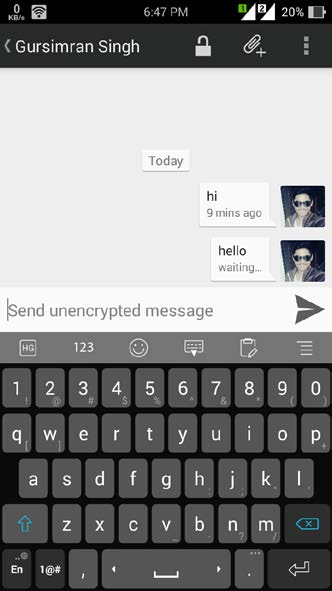
\includegraphics[scale=0.3]{input/images/s3.png}
\caption{Sending Message Test}
\end{figure}
\item Sending an encrypted message/file to a contact using OMEMO (Multi-End Message and
Object Encryption).\\
\noindent \textbf{Description:}
A registered user should be able to send an encrypted message to a contact.\\
\noindent \textbf{Precondition:}
The user must already be registered with an email address and password and internet is
connected and OMEMO encryption is selected.\\
\noindent \textbf{Test Steps:}
\begin{itemize}
\item Open the app.
\item Click on the name of the contact to send a message.
\item Select encryption method to OMEMO.
\item Select the file to send.
\item Click on the send button
\end{itemize}
\noindent \textbf{Expected Result:}
The file/image is sent successfully with an encryption lock sign below the message.\\
\begin{figure}[ht]
\centering
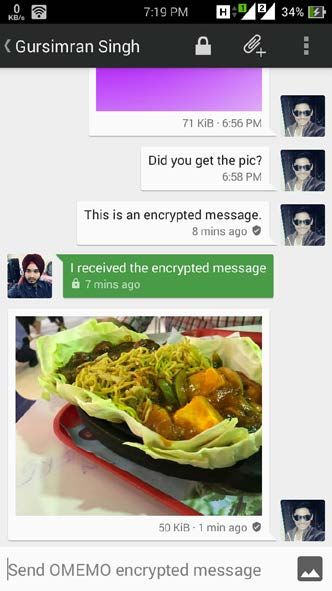
\includegraphics[scale=0.3]{input/images/s4.png}
\caption{Sending Encrypted text/file Test}
\end{figure}
\item Sending and receiving messages in a group\\
\noindent \textbf{Description:}
A registered user should be able to send an encrypted message in a group.\\
\noindent \textbf{Precondition:}
The user must already be registered with an email address and password and internet is
connected.\\
\noindent \textbf{Test Steps:}
\begin{itemize}
\item Open the app.
\item Click on the name of the group to send a message.
\item Click on the send button
\end{itemize}
\noindent \textbf{Expected Result:}
The message is sent successfully..\\
\begin{figure}[ht]
\centering
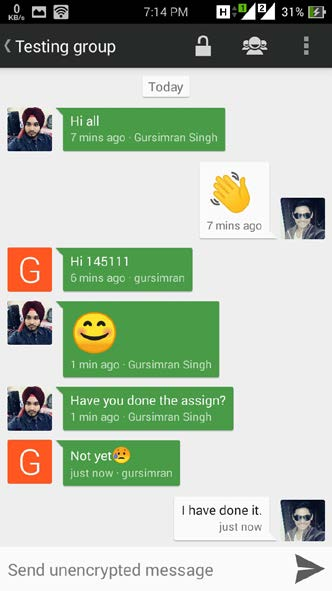
\includegraphics[scale=0.3]{input/images/s5.png}
\caption{Messaging in Group Test}
\end{figure}
\end{enumerate}
\subsection{Paigaam Assistant(Chatbot)}
\begin{itemize}
\item
 Sending queries to the chatbot as a student and getting the required results.
\noindent \textbf{Description:}
A registered student should be able to send queries to the chatbot and get the appropriate
results.\\
\noindent \textbf{Precondition:}
The user must already be registered with an email address and password and internet is
connected.\\
\noindent \textbf{Test Steps:}
\begin{itemize}
\item Open the app and click on Paigaam-Assistant from the contact list.
\item Type the below query and press send button:
\begin{enumerate}
\item Hi
\item My Fee Status
\item My attendance
\item My marks in 7th semester
\item Teacher details
\end{enumerate}
\end{itemize}
\noindent \textbf{Expected Result:}
The chatbot should reply with the correct message corresponding to the query.\\

\begin{figure}[ht]
\centering
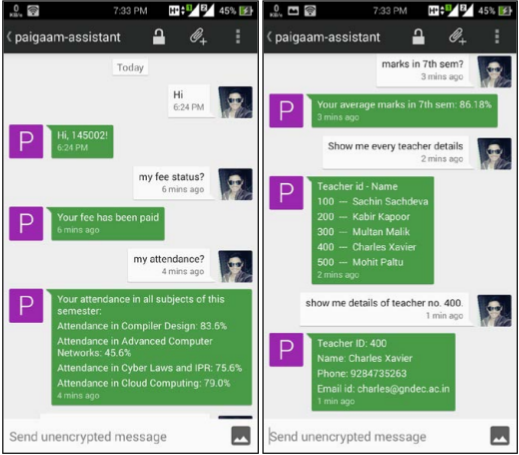
\includegraphics[scale=0.3]{input/images/s11.png}
\caption{Testing Paigaam Assistant as a Student}
\end{figure}
\item
Sending queries to the chatbot as a teacher and getting the required results.\\
\noindent \textbf{Description:}
A registered teacher should be able to send queries to the chatbot and get the appropriate
results.\\
\noindent \textbf{Precondition:}
The teacher must already be registered with an email address and password and internet is
connected.\\
\noindent \textbf{Test Steps:}
\begin{itemize}
\item Open the app and click on Paigaam-Assistant from the contact list.
\item Type the below query and press send button:
\begin{enumerate}
\item Hi
\item My courses
\item List students under course number 200
\end{enumerate}
\item Click on the send button
\end{itemize}
\noindent \textbf{Expected Result:}
The chatbot should reply with the correct message corresponding to the query.\\
\begin{figure}[ht]
\centering
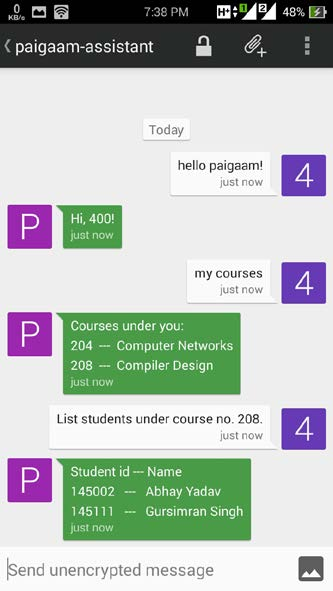
\includegraphics[scale=0.3]{input/images/s12.png}
\caption{Testing Paigaam Assistant as a Teacher}
\end{figure}
\end{itemize}
\subsection{Paigaam Web Client}
\begin{itemize}
\item
Login and messaging
\noindent \textbf{Description:}
A registered user should be able to login into the app and send messages to contacts.\\
\noindent \textbf{Precondition:}
Internet should be connected and modern browser such as Chrome/Firefox should be used.\\
\noindent \textbf{Test Steps:}
\begin{itemize}
\item Open a web browser and open the URL https://ambivert.me/jsxc/example/
\item Enter the registered ID and password
\item Click on Login Button
\item Once logged in, click on a contact name
\item Send message.
\end{itemize}
\noindent \textbf{Expected Result:}
The user is successfully logged in and the main interface of the app is shown.\\

\begin{figure}[ht]
\centering
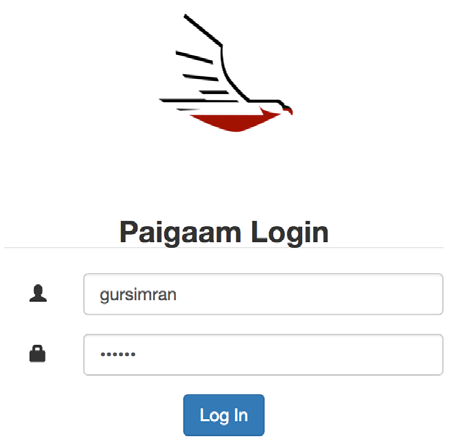
\includegraphics[scale=0.4]{input/images/s21.png}
\caption{Paigaam Login Test}
\end{figure}
\newpage
\begin{figure}[ht]
\centering
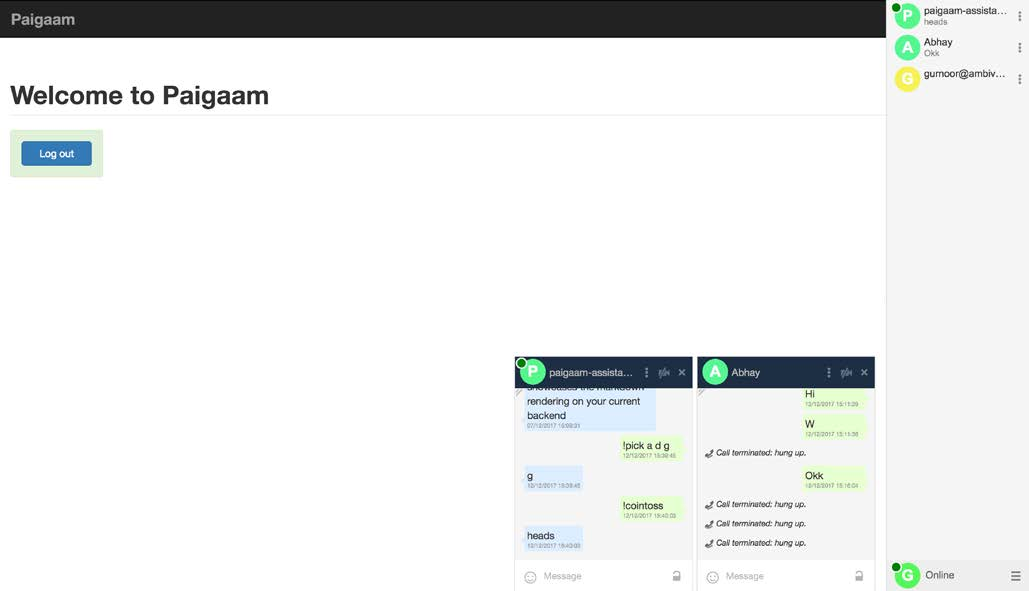
\includegraphics[scale=0.4]{input/images/s22.png}
\caption{Paigaam Login Success Test}
\end{figure}
\item
Video Chat\\
\noindent \textbf{Description:}
A registered user should be able to Video chat with a contact.\\
\noindent \textbf{Precondition:}
Internet should be connected and modern browser such as Chrome/Firefox should be used.\\
\noindent \textbf{Test Steps:}
\begin{itemize}
\item Open a web browser and open the URL https://ambivert.me/jsxc/example/
\item Enter the registered ID and password
\item Click on Login Button
\item Once logged in, click on a contact name
\item Click on a contact name and then on the video chat button
\end{itemize}
\noindent \textbf{Expected Result:}
The video chat request is sent to the contact and video streaming is possible..\\
\begin{figure}[ht]
\centering
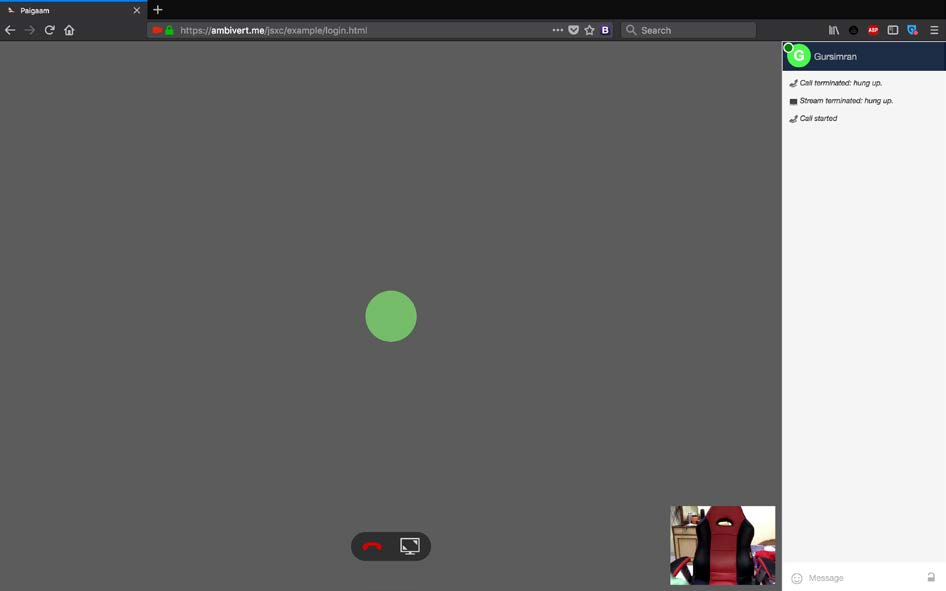
\includegraphics[scale=0.3]{input/images/s31.png}
\caption{Video Chat Test}
\end{figure}
\begin{figure}[ht]
\centering
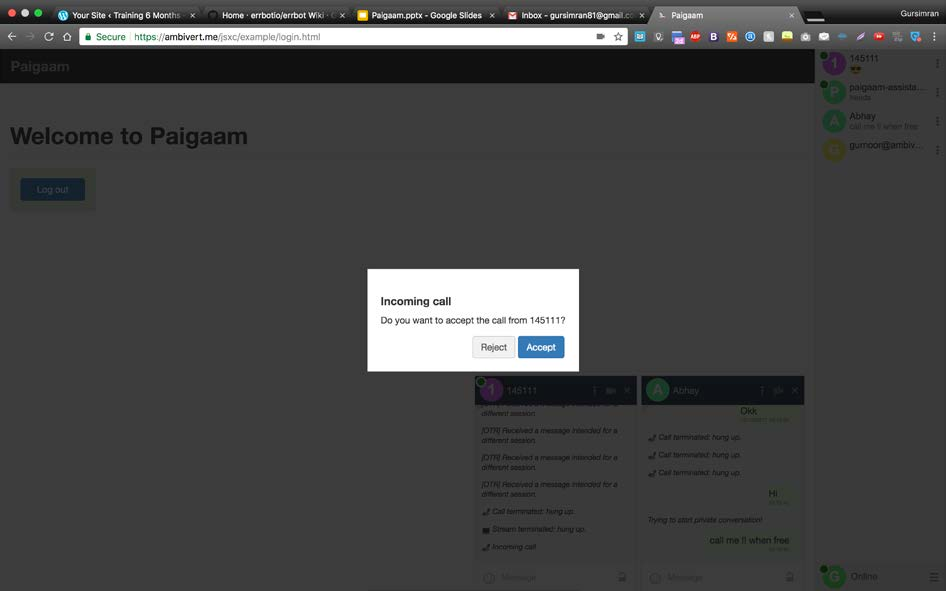
\includegraphics[scale=0.3]{input/images/s32.png}
\caption{Chat Accepting Video Chat Test}
\end{figure}
\begin{figure}[ht]
\centering
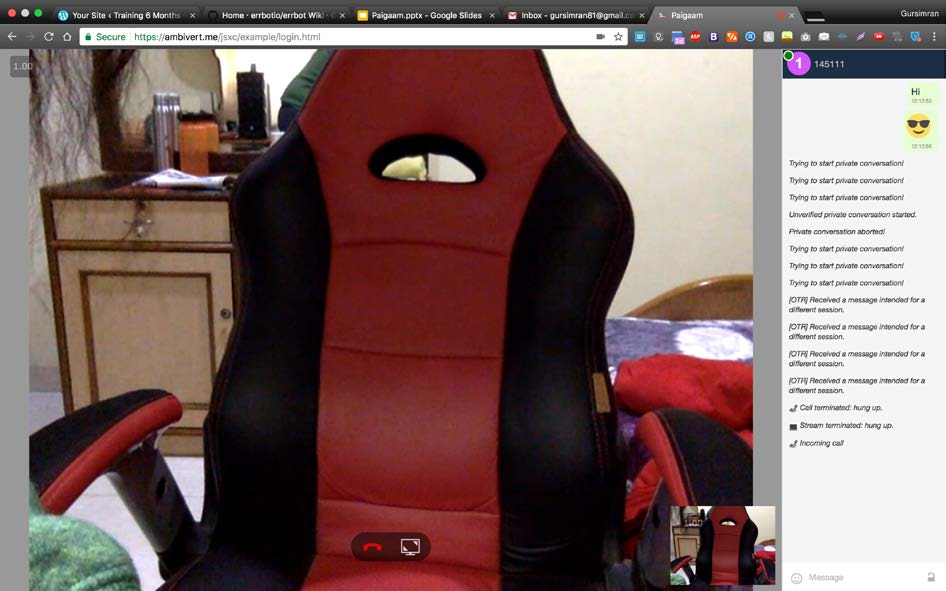
\includegraphics[scale=0.3]{input/images/s33.png}
\caption{Video chat Accepted Test}
\end{figure}
\end{itemize}